\documentclass[12pt]{article}
\usepackage[pdftex]{graphicx}
\usepackage{paralist}
\usepackage{pdfpages}
\usepackage{enumitem}
\usepackage{hyperref}
\usepackage{csquotes}
\usepackage[margin=1in]{geometry}
\usepackage{times}
\usepackage{soul}
\usepackage{setspace}
\singlespacing



\usepackage{MnSymbol}
 \usepackage[american]{babel}

  \usepackage[style=apa,sortcites=true,sorting=nyt,backend=biber]{biblatex}
  \DeclareLanguageMapping{american}{american-apa}
  \addbibresource{bib.bib}

\newcommand{\HRule}{\rule{\linewidth}{0.5mm}}

\usepackage{titlesec}
\titleformat{\section}
  {\normalfont\Large\bfseries}{\thesection}{1em}{}[{\titlerule[0.8pt]}]

\renewcommand\thesection{\Alph{section}}


\begin{document}
\begin{titlepage}
\begin{center}


\textsc{\LARGE Bucknell University}\\[1.5cm]
\textsc{\large A Proposal to}\\[0.5cm]
\textsc{\Large  Program for Undergraduate Research}\\[0.5cm]

% Title
\HRule \\[0.4cm]
{ \huge \bfseries Improving Computer-Mediated Decision Making via Physiological Signals from Wearable Sensors \\[0.4cm] }

\HRule \\[1.5cm]

% Author and supervisor
% \noindent
% \begin{minipage}{0.4\textwidth}
% \begin{flushleft} \large
\emph{Student Author:}\\
Xiaoying \textsc{Pu}\\
Class 2017\\
Box C1657, (570)360-0243\\
xp002@bucknell.edu\\
BU ID: 11384971\\
% \end{flushleft}
% \end{minipage}

% \begin{minipage}{0.4\textwidth}
% \begin{flushright} \large

\vspace{10pt}
\emph{Advisor:} \\
Dr.~Evan \textsc{Peck}\\
Department of Computer Science\\
emp017@bucknell.edu
% \end{flushright}
% \end{minipage}

\vfill

% Bottom of the page
{\large \today}
\vspace{40pt}
\end{center}
{\large Advisor Signature \underline{\hspace{5cm}} \vspace{20pt} }\\
{\large Student Signature \underline{\hspace{5cm}}}

\end{titlepage}

\section{Project Description}\label{project-description}

\subsection{Background}\label{background}

Given that wearable sensors could inform computers of our state of mind, we propose to build an ``attentive'' computer system that could present us with decisions when we are best equipped to handle them. 



\begin{enumerate}
\def\labelenumi{\noindent \alph{enumi}.}
\itemsep0pt\parskip0pt\parsep0pt
\item{\it Decision making and cognitive overload}\\
  People tend to make bad decisions when they are under stress or heavy workload. 
  According to {\it Thinking, Fast and Slow}, our thought process could be explained by two systems: ``System 1'' is fast and instinctive, and ``System 2'' is deliberate and logical. When performing complicated tasks that occupy the limited processing capability of ``System 2'', people tend to make decisions based on immediate affection instead of logic and cognition. This conflict of affect and cognition in decision-making is presented through a popular experiment involving a choice between chocolate cake and fruit salad \parencite{Fedorikhin2014}. When the experiment respondents were asked to memorize long numbers, their mind occupied, they tended to choose unhealthy chocolate cakes over the fruit salad. 


  \hspace{15pt} In the real world, people face decisions more serious than choosing a desert. Bad decisions made in unsuitable cognitive conditions can have serious consequences. For instance, air-traffic controllers' tasks often entail high cognitive workload involving information processing and logic reasoning. In 2002, a controller, Peter Nielsen, was under heavy workload, and his mistake led to the \"{U}berlingen mid-air collision that claimed 71 lives. There is a need to detect the user's stress level and apply that information to promote decision-making.\\

\item{\it Technology has become a mediator for decision-making}\\
As technology becomes more integrated in people's lives, decisions are often taken in context of some kind of computer; decision-making has become an important aspect in Human-Computer Interaction (HCI) \parencite{Zhou2015}.
Important mediators as they are, computers generally understand users poorly. By the mere means of keyboards or touch screens, much of the relational information present in social contexts is not perceived by computers. Studies have shown that interruption (by computers) at bad moments could increase stress levels and decrease performance \parencite{Carton2009}. 
Computers could do better in mediating decision-making by gaining a better understanding in users' state of mind, and they should be able to choose better moments to present the user with complex problems like choices.\\


\item{\it Wearable physiological sensor as solution}\\
Recent studies have made initial attempts to utilize physiological signals and to use biofeedback to promote better decision making \parencite{Carroll2013, Zhou2015}. 
  Stress could manifest as many characteristic physiological signals, such as electrodermal activities (EDA), heart-rate, skin temperature and pupil size. 
  Some of these signals could now be acquired through a variety of burgeoning wearable sensors, such as wristbands and headbands. We could process those physiological signals to decide whether the user is in a stressed state or not. There are several advantages that make wearable sensors suitable for mediating decision-making \parencite{Peck2014}:
  \begin{enumerate} 
  \itemsep0pt\parskip0pt\parsep0pt
    \item As opposed to traditional electroencephalography (EEG), wearable sensors are portable enough to be used in everyday  environment, where decisions are made.
    \item Users can provide input to computers via wearable sensors, without interrupting their tasks and thought processes.
    \item Physiological signals provide computers with the previously unaccessible  information that we naturally pick up through social cues.
  \end{enumerate}
\end{enumerate}

\subsection{This Project}\label{this-project}


Starting from a big concept, we will combine pre-existing technologies in an innovative way. As shown in Figure \ref{figure:mindmap}, this project could be encapsulated as a biocybernetic loop, which utilizes physiological information to adapt the computer system the user is interfaced with. A senior design team is currently working on a program framework that could determine whether a user is stressed or not. This part of the system (signal analyzer in Figure \ref{figure:mindmap}) takes physiological signals as input and judges the state of mind of the user. The output of the signal analyzer will drive our decision making delivery system.

We will also work with people at Bucknell and beyond. For instance, Professor Joaquin Gomez-Minambres in Economics Department specializes in behavioral economics and decision-making, and has expressed interest in collaborating on this project. Professor Erin Solovey at Drexel University is an expert in adaptive physiological systems and could provide insight into processing physiological data.

\begin{figure}[h]
\centering
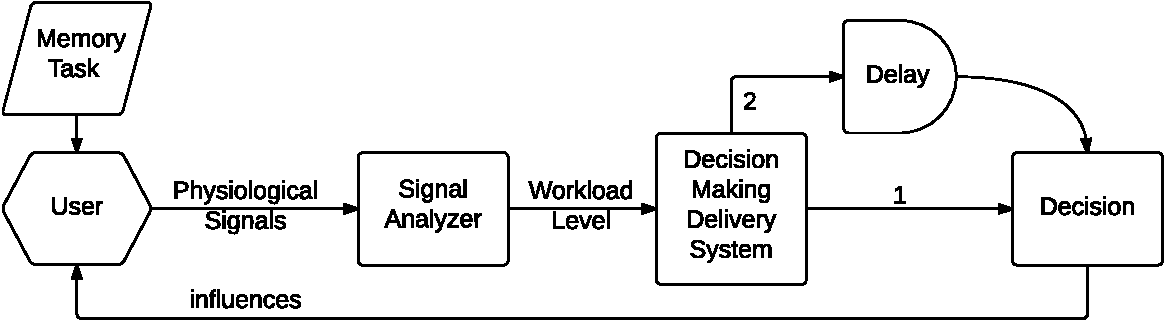
\includegraphics[width=0.9\textwidth]{hci_mindmap.pdf}
\caption{This project viewed as a biocybernetic loop.}
\label{figure:mindmap}
\end{figure}




\subsection{Methods}\label{methods}


In order to assess the effectiveness of our system, we will create controlled stress level and decision-making process. Established psychology tasks will be used to manipulate stress level; examples include the n-back task or digit span. We will also incoporate decision-making questions that have been validated by the psychology community. Physiological signals will be acquired through Empatica E4. It is a wristband that contains a heart-rate sensor, 3-axis accelerometer, skin temperature + heat flux sensor, and electrodermal activity sensor. We will conduct within-subjects experiments, meaning the same group of participants will be presented with two decision-making systems:
\begin{enumerate}
\itemsep1pt\parskip0pt\parsep0pt
\item One that deliver decisions immediately, while the participant is still under stress (the path 1 in Figure \ref{figure:mindmap}). 
\item One that deliver decisions at ``good moments'', a judgment made based on the participant's physiological signals. If the user is stressed, decisions will not be presented immediately (path 2).
\end{enumerate}



\subsubsection{Time Line}
\begin{itemize} 
\itemsep0pt\parskip0pt\parsep0pt
\item Weeks 1-4: Construct experimental platform and validate of physiological measures.
\item Weeks 5-6: Perform pilot study and review experimental procedures.
\item Weeks 7-8: Conduct decision-making experiment with participants.
\item Weeks 9-10: Analyze data and compile a research paper.
\end{itemize}


\subsection{Anticipated Outcome}\label{anticipated-outcome}
We expect to:
\begin{inparaenum}[\itshape 1\upshape)]
\item
  assess how well we can predict a good or bad decision based purely on physiological signals;
\item 
  evaluate whether we can improve decision making by choosing more opportune moments to deliver decisions;
\item
  write a research paper and
\item
  submit for ACM Conference on Human Factors in Computing Systems (CHI) 2016. CHI is the most prestigious venue in HCI.
\end{inparaenum}






\section{Research Environment}\label{research-environment}

I will work closely with Professor Peck throughout the research period.
Professor Peck will be present and available over the summer, and there
will be daily discussions and weekly summarizations. We will collaborate
on multiple levels, from generating new ideas to coding. Because of the
digital nature of this project, Professor Peck has planned on a
practical project management system that includes GitLab, Google Drive, Slack and Trello. This research will be conducted in Dana or Breakiron labs.
    
 \printbibliography
 
%\begingroup
%\setstretch{0.8}
%\setlength\bibitemsep{0pt}
%\bibliographystyle{plain}
%\bibliography{bib.bib}
%\endgroup




\end{document}
